\documentclass[11pt, a4paper]{article}
\usepackage[utf8]{inputenc}
\usepackage{fullpage}
\usepackage{graphicx}
\usepackage{markdown}
\usepackage[hidelinks]{hyperref,xcolor}
\renewcommand\UrlFont{\color{blue}\rmfamily}

\usepackage[backend=biber]{biblatex}
\addbibresource{library.bib}
\title{Project Plan\\Remote Water Sensing using UAVs}
\author{Robin \textsc{Westerik}}

\newcommand{\supervisors}{Jan \textsc{Bollen}\\Harry \textsc{Futselaar}}
\newcommand{\timePeriod}{February 2022 - June 2022}
\newcommand{\resourcesPlanned}{800 hours (40h per week)}
\newcommand{\homepage}{\url{https://github.com/organizations/remotewatersensing/}}
\date{\today}

\makeatletter{}

\begin{document}

\begin{titlepage}
  	\newcommand{\HRule}{\rule{\linewidth}{0.3mm}}
	\center
	\textsc{\LARGE Saxion University of Applied Sciences}\\[1.5cm]
	\textsc{\Large International Water Technology}\\[0.5cm]
	\textsc{\large Applied Computer Science Graduation Project}\\[0.5cm]
	\HRule\\[0.4cm]
	{\huge\bfseries \@title}\\[0.4cm]
	\HRule\\[1.5cm]

	%Author(s)
	\begin{minipage}{0.4\textwidth}
		\begin{flushleft}
			\large
			\textit{Author(s)}\\
			\@author % Your name
		\end{flushleft}
	\end{minipage}
	~
	\begin{minipage}{0.4\textwidth}
		\begin{flushright}
			%\large
			%\textit{Supervisor(s)}\\
			%\supervisors
		\end{flushright}
	\end{minipage}
	
% 	If you don't want a supervisor, uncomment the two lines below and comment the code above
% 	{\large\textit{Author(s)}}\\
% 	\@author % Your name

	%Date
	\vfill\vfill
		{\large\today}
    \vfill\vfill
    
    \footnotesize{Time period: \timePeriod}
    \\[0.3cm]
    \footnotesize{Resources planned: \resourcesPlanned}
    \vfill
    \homepage
    
    \vfill
    
    \begin{tabular}{ | l | l | l | l |}
    \hline
    \textbf{Version} & \textbf{Date of change} & \textbf{What is changed?} & \textbf{The reason for the change} \\ \hline
    0.1 & 03-02-2022 & templating & \\
    0.2 & 03-02-2022 & added project result & \\
    0.21 & 07-02-2022 & edited project result & added research question\\
    0.3 & 07-02-2022 & added project activities &\\
    0.4 & 07-02-2022 & added project boundaries &\\
    0.5 & 08-02-2022 & added interim results, quality &\\
    \hline
\end{tabular}
	
	\vfill\vfill
	
\includegraphics[width=0.4\textwidth]{./saxionlogo.png}
	\vfill
	 
	\vfill
	
\end{titlepage}


\tableofcontents
\pagebreak

\section{Background}
This project proposal has been brought forward by an idea of the International Water Technology lectorate at the Saxion University of Applied Sciences. The project will be carried out in collaboration with PERNAM JSC, a specialist in water treatment solutions in Vietnam. They are specialized in the design, engineering, and construction of water treatment technologies for groundwater, surface, and brackish water. Ton Duc Thang University, a public research university located in Ho Chi Minh City, will further accommodate the project when possible by providing expert advice and practical necessities. 

As this project will be a first of potential following projects, emphasis is laid on developing an open source and well documented foundation so that future parties can build on this project in the future. Completing this project could be a start of providing smarter water sensing solutions which in turn could benefit current water filtration solutions of Pernam as well as help with the water availability issues around Ho Chi Minh City.

\section{Project Result}
Monitoring surface level water could be vital for providing feedback to water filtration solutions. Having more autonomous ways to monitor the water quality will lead to less man hours spent manually measuring the water.

The objective during this graduation project is to explore new ways in which water can be autonomously monitored by using unmanned aerial vehicles (drones). While it is not possible to know in advance exactly what the end product would entail, it would allow users to measure various water quality variables across an area by using unmanned aerial vehicles and various different water quality sensor concepts.

Future projects could mature by for example improving a specific sensor concept or by using past data to automatically determine the best filtration settings.

\subsection{The Research Problem}

The research question that the project will make an attempt to answer is as follows:\vspace{3mm}

\large{What is the best way to measure the surface water quality using drones in Vietnam?}\vspace{3mm}\\
\normalsize
To elaborate, this research question can be deconstructed as following:
\subsubsection{The best way}
The best way is dependent on a number of features that are important to the sponsor. These features naturally include accuracy, time, cost, and practicality, and will be discussed during the design sprint (\ref{sprint:design}).

\subsubsection{Surface water quality}
Surface water is any body of water above ground, including streams, the ocean, rivers, lakes, wetlands, reservoirs, and creeks.\cite{surfacewater}

Water quality refers to the chemical, physical, and biological characteristics of water based on the standards of its usage. These water standards will be defined during the analyze sprint (\ref{sprint:analyze}).

\subsubsection{Using drones}
While there are a lot of different existing ways to measure the water quality, this project will focus solely on using unmanned aerial vehicles, as elaborated in the project boundaries (\ref{projectboundaries}).

\subsubsection{In Vietnam}
It can be concluded that certain sensoring strategies are effective in different climates and landscape. This project will focus on water sensoring in Vietnam, specifically in areas where PERNAM JSC are active. These areas will be defined during the analyze sprint (\ref{sprint:analyze}).

\section{Project Activities}
The project consists of several sprints. These sprints will have time boxed periods, and usually last two to four weeks. Sprints can intertwine with each other if necessary. Each sprint will be managed using a kanban \cite{kanban} board with three columns: To-Do, In-Progress and Done. These sprints are heavily influenced by competences given by the project assignment. \cite{assignmentform}

\subsection{Analyze} \label{sprint:analyze}
Existing water sensoring solutions and suitable drones will be analyzed. Water quality standards used will also be analyzed. Literature will be reviewed, and findings of which will be contained in a preliminary research report.  It is important to note that this document can be extended during other sprints, when new info related to the project is found. A change log as well as git \cite{git} will keep track whenever this document is edited.

\subsection{Design} \label{sprint:design}
An overview of the working architecture will be designed, along with several prototypes of ways to measure the water quality using drones. The result of which will be contained in the design report. This design report will reference a lot of findings from the preliminary research report. There will also be a lot of communication between the sponsor and the project author to discuss the focus of these designs. \\

To begin, effective variables to measure water quality will be selected. Sensors will be selected to measure these variables based on their accuracy and capability to mount on a drone. A suitable drone will be chosen using a morphological overview. Configurations of these sensors on the drone will be designed and illustrated. 

\subsection{Realise} \label{sprint:realise}
Multiple prototypes will be realized within the given time and budget. Mounting will be made if necessary. Software will be written to fly the drone and to read (and possibly transmit) sensor data. This software will include documentation befitting industry standards.\\

During this sprint, no new reports will be written. Whenever there is an issue with a design, the design report can be edited. A change log as well as the git version control system \cite{git} will keep track of these edits.

\subsection{Research}
From each of these prototypes, several quantitative and qualitative features will be tested. These features include accuracy, speed, and cost. The summary of this descriptive, non-probabilistic research is written down in the final research report.

\subsection{Professionalise}
If there is time left, the most compelling prototype will be refined to a minimum viable product (MVP). This minimum viable product can be derived from one prototype or mixed together from multiple prototypes. The process will be similar to the realize sprint \ref{sprint:realise}, with the final design being added in the design report.

\section{Project Boundaries} \label{projectboundaries}

\section{Interim Results}

\section{Quality}

\section{Project Organization}

\section{Planning and Scheduling}

\section{Costs and Benefits}

\section{Risks}

\begin{figure}[h]
    \center
    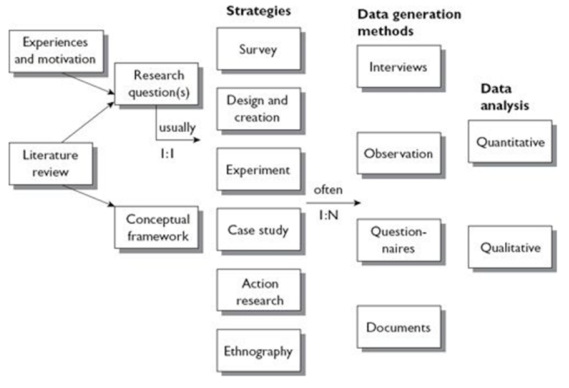
\includegraphics[width=0.5\textwidth]{research-strategies.png}
    \caption{Research strategies \cite{oates2005researching}}
    \label{fig:research_strategies}
\end{figure}

% References
\printbibliography 
\pagebreak
%Remove excerpt when publishing

\markdownInput{roelgrit.md}
\end{document}
